\documentclass[a4paper,fleqn]{cas-sc}

\usepackage[numbers,sort&compress]{natbib}
\usepackage{amsmath,mathtools}
\usepackage{booktabs}
\usepackage{multirow}
\usepackage{threeparttable}
\usepackage{enumitem}
\usepackage{xspace}
\usepackage{float}
\usepackage{placeins}
\usepackage{caption}
\usepackage{graphicx}
\graphicspath{{../figures/}}
\usepackage{xcolor}

\newcommand{\acro}[1]{\textsc{\MakeLowercase{#1}}\xspace}
\newcommand{\FX}{\acro{FX}}
\newcommand{\CLOB}{\acro{CLOB}}
\newcommand{\AMM}{\acro{AMM}}
\newcommand{\HFMM}{\acro{HFMM}}
\newcommand{\ABM}{\acro{ABM}}
% Marker for material that requires the new simulation runs.
\newcommand{\TODO}[1]{\textcolor{red}{\textbf{[TO BE COMPLETED: #1]}}}

\ExplSyntaxOn
\cs_set:Npn \__first_footerline: {}
\ExplSyntaxOff
\begin{document}
\let\WriteBookmarks\relax

\shorttitle{Standing liquidity backstops in FX markets}
\shortauthors{D. Voinov and P.\,P. Lukianchenko}

\title[mode=title]{Standing Liquidity Backstops in Foreign Exchange Markets: A Resource Matched Comparison of Facility Designs}

\author[1]{David Voinov}[orcid=0009-0006-7420-2942]
\cormark[1]
\credit{Conceptualization, Methodology, Software, Formal analysis, Visualization, Writing -- original draft}
\affiliation[1]{organization={HSE University, Faculty of Computer Science, Bachelor's Programme ``Data Science and Business Analytics''},
                city={Moscow}, country={Russia}}

\author[2]{P.\,P. Lukianchenko}[orcid=0000-0002-1022-6041]
\credit{Conceptualization, Supervision, Writing -- review and editing}
\affiliation[2]{organization={Trusted AI Research Center, Ivannikov Institute for System Programming of the RAS (ISP\,RAS)},
                city={Moscow}, country={Russia}}

\cortext[cor1]{Corresponding author: ddvoinov@edu.hse.ru}

\nonumnote{JEL classification: F31, G15, G28, C63}

\begin{abstract}
Dealer supplied liquidity in foreign exchange markets deteriorates at the moment it is most valuable, because dealers widen their quotes and withdraw when volatility, funding stress and inventory risk rise together. A standing facility obliged to quote throughout a crisis would cushion the resulting dislocation, but somebody has to hold the capital that keeps it open and absorb the losses it takes while doing so, which makes the terms on which such a facility is funded the substantive question. We study those terms in an agent based model of a dealer intermediated spot market where dealers withdraw endogenously and a reserve priced facility is overlaid as a counterfactual venue. The facility reduces the amplitude of the crisis dislocation while leaving the normalised speed of recovery largely unchanged, and the order flow that migrates to it is the flow the dealer sector is least willing to hold, so its losses accumulate in the states where its availability matters most. A venue that prices off its reserves cannot defend itself by widening and does not recover those losses from fee income, while the fee that would improve provider economics weakens the backstop delivered. What the model describes is a funded institution whose subsidy can be measured, and we trace the frontier along which resilience is bought at the cost of keeping that institution solvent.
\end{abstract}

\begin{keywords}
foreign exchange market \sep liquidity resilience \sep market design \sep standing liquidity facility \sep automated market maker \sep agent based model
\end{keywords}

\maketitle

\section{Introduction}
\label{sec:intro}

Foreign exchange (\FX{}) liquidity is supplied primarily by a concentrated set of strategic dealers that continuously adjust quotes in response to volatility, order flow imbalances, and balance sheet constraints \citep{rime2013,bis2025,Brunnermeier2009}. In calm conditions this delivers tight spreads and deep books, but under stress dealer capacity deteriorates quickly, producing wider spreads, thinner books, and slow post shock recovery \citep{ranaldo2022,karnaukh,huang2024,bollerslev1994}. Because this fragility concentrates exactly when liquidity is most valuable, what matters is not only the average level of liquidity but how the market behaves when dealer intermediation fails.

The fragility of dealer intermediation invites an institutional remedy in the form of a standing facility that is funded in advance and obliged to quote throughout a crisis, and the questions such an arrangement raises are financial before they are technological. Somebody has to hold the capital that keeps the facility open, absorb the losses it takes while doing so, and settle what it charges for the service, and those terms determine both whether the arrangement can exist and how much resilience the money buys. The question is also timely because AI driven trading and automated liquidity management make machine mediated market making increasingly relevant for stress episodes in electronic \FX{} markets.

Automated market makers offer one way of organising such a facility, since an \AMM{} prices every trade off a fixed function of its reserves and so quotes mechanically at whatever reserves it holds, without the discretion a dealer exercises when it decides to step away \citep{mohan}. That property is narrower than it first appears, because what the contract fixes is the pricing rule at given reserves and nothing at all about the willingness of liquidity providers to leave their capital in the pool. A facility of this kind can be drained on one side, can become severely imbalanced, and can in principle be abandoned by the providers who fund it, and its pool mid reprices only through arbitrage and therefore lags a continuously requoted dealer market \citep{park2023,milionis2022}. Reserve pricing is also not the only arrangement carrying a commitment to remain available, since a committed dealer of last resort quoting a single spread, or a passively managed order book facility, would serve the same function by different means. Any comparison that adds such a facility to an otherwise unchanged dealer market consequently measures three things at once, namely the arrival of additional committed capital, the obligation to stay open, and the particular pricing rule, and attributing the whole of that combination to the pricing technology would overstate what the exercise establishes.

We study these questions in an agent based model of a multi venue \FX{} market where dealers withdraw endogenously in response to their own losses, inventory, funding conditions and the state of market wide liquidity, and where a reserve priced facility is overlaid as a counterfactual venue. The comparison we are able to run is not resource matched, since the treatment arm carries committed capital the control arm lacks, and we take that limitation seriously enough to bound the pricing channel from one side. Disabling the cost aware routing that steers flow toward the facility, and replacing it with a fixed share split, leaves a facility that does nothing except stay open and absorb whatever it is given, which isolates the contribution of availability from the contribution of the schedule. The fully resource matched design that would complete the separation, together with the capital and subsidy conventions it requires, is set out in Section~\ref{sec:conc}.

The analysis is organised around four claims, each connecting the resilience the facility delivers to the terms on which it is financed. A facility that remains available lowers the amplitude of the post shock dislocation, while the normalised speed at which the spread returns toward its pre shock level is left unaffected, so the resilience gain is properly described as an effect on amplitude (H1). Order flow migrates toward the facility as dealers retreat, and because the orders that migrate are those the dealer sector is least willing to hold, the facility accumulates adversely selected exposure in precisely the states where its availability is most valuable (H2). The price advantage it offers is confined to large trades, since a flat reserve schedule is crossed by a steeply rising dealer cost only in the upper tail (H3). The facility does not pay for itself at any fee we examine, and the fee that improves the economics of its providers weakens the backstop it delivers, which traces a frontier along which resilience is purchased with subsidy (H4).

\section{Related literature and contribution}
\label{sec:lit}

Theoretical work on the coexistence of order books and automated venues has already characterised how traders sort between the two and how that sorting feeds back into liquidity provision, most completely in the equilibrium analysis of \citet{coexisting}, and the routing rule we employ is a reduced form counterpart of that mechanism with none of its equilibrium discipline. Empirical work has measured the relative quality of the two venue types directly, with \citet{barbon2023} documenting that fixed costs penalise small trades while decentralised venues compete more effectively for large ones, and with \citet{lehar2024} characterising equilibrium in Uniswap pools together with the conditions under which an automated venue dominates a limit order market. We treat the first of those findings as a target our model should reproduce without having been calibrated to it, since our calibration touches only calm state \FX{} moments and never any crossover, so the correspondence serves as a check on the mechanism and carries no claim of priority.

The economics of liquidity supply on such venues has likewise been endogenised elsewhere. \citet{hasbrouck2024dex} show that higher fees can raise volume because fee revenue attracts inventory and inventory lowers price impact, an argument extended to concentrated liquidity by \citet{hasbrouck2025cl}, while \citet{milionis2022} formalise the loss versus rebalancing that passive providers bear whenever the rate moves. That literature bears directly on the subsidy accounting we present below, and it also identifies the sharpest limitation of our design, since holding reserves fixed suppresses the feedback running from provider compensation back to the quantity of liquidity supplied. Studies asking whether automated market making would improve conventional markets, notably \citet{foley2023} and \citet{malinova2023}, come closest to our question in spirit, though they address equity and traditional venues and leave dealer intermediated \FX{} unexamined.

Our contribution against this background is a modest one, since each element we combine is individually familiar, and what the paper adds is the combination of endogenous dealer withdrawal, a standing facility, and an explicit accounting of what keeping that facility open costs its providers, assembled in a dealer intermediated \FX{} setting and evaluated on resilience and on the terms under which such a facility could be financed. The model is abstract in the sense of \citet{gilbert2008}, built to expose a mechanism and to support reasoning about rules and institutions without pretending to be a facsimile of the spot market, and we are correspondingly explicit in Section~\ref{sec:calib} about which quantities are disciplined by data and which are choices we have made.

\section{Model}
\label{sec:model}

The market is modelled in event time over a common state \((S_t,\sigma_t,c_t,\ell_t)\) of fair price, volatility, funding cost, and systemic liquidity, with signed order flow imbalance \(OFI_t\) also tracked. A dealer \CLOB{} and a standing facility operate in parallel, and a population of nondealer traders generates background flow. The nondealer classes, their activation rules and their order generation rules are given in Table~\ref{tab:agent_rules}.

\subsection{Dealers and endogenous withdrawal}

The \CLOB{} is intermediated by five strategic dealers that differ slightly in spread floors and depth scales. Higher volatility \(\sigma_t\) or funding stress \(c_t\) causes a dealer to widen its spread to cover the higher risk of quoting \citep{stoll1978,kyle1985,glosten1985}, while one sided order flow or inventory accumulation causes it to show less depth.

\paragraph{Dealer state variables and withdrawal rule.}
The supplement collects the reduced form objects referenced in the main text. Dealer quoting uses the AMM adjusted order flow, inventory, and liquidity modifiers \((\widetilde{OFI}_t,\widetilde{\iota}_t,\widetilde{\ell}_t)\),
\begin{equation}
s^{*}_{j,t}=\alpha_0+\alpha_1 \sigma_t+\alpha_2 c_t+\alpha_3 |\widetilde{OFI}_{t}|,
\qquad
d^{*}_{j,t}=\max\left\{d_{\min},\left(d_0-d_1 \sigma_t-d_2 c_t-d_3 |\widetilde{OFI}_{t}|-0.1|I_{j,t}|\widetilde{\iota}_t\right)\widetilde{\ell}_t\right\}.
\end{equation}
The composite withdrawal score is
\begin{equation}
\Xi_{j,t}=0.40 L_{j,t}+0.12 V_t+0.05 F_t+0.22 I^{risk}_{j,t}+0.22 O_t+0.32 D_t+0.10 A_t+\Psi_t,
\end{equation}
with
\begin{equation}
L_{j,t}=\min\left\{3,\frac{\mathrm{EWMA\ loss}_{j,t}}{\theta_{loss}}\right\},\quad
V_t=\min\left\{2.5,\frac{\sigma_t}{\sigma_0}-1\right\},\quad
F_t=\min\left\{2.5,\frac{c_t}{c_0}-1\right\},
\end{equation}
\begin{equation}
I^{risk}_{j,t}=\min\left\{1.5,\frac{\max(|I_{j,t}|,|q_{j,t}|)}{1.5\,\bar q_j}\right\},\quad
O_t=\min\left\{2,|OFI_t|\right\},\quad
D_t=\min\left\{1.5,1-\ell_t\right\},\quad
A_t=\min\left\{1.5,\mathrm{AMM\ support}_t\right\}.
\end{equation}
The shock term is \(\Psi_t=0.85\lambda_t+0.30\tau_t+0.25\omega_t\). Dealers move from active/defensive to withdrawn when \(\Xi_{j,t}\ge \bar\Xi\), from active to defensive when \(\Xi^{def}\le \Xi_{j,t}<\bar\Xi\), and back to active when \(\Xi_{j,t}\le \underline\Xi\). Reentry after withdrawal also requires \(\ell_t\ge 0.55\).

In spot \FX{}, withdrawal is interpreted broadly as wider last look rejection, reduced internalization, or quote cancellation, all of which reduce available liquidity. Because withdrawal is triggered by a dealer's own state rather than imposed by hand, liquidity droughts emerge endogenously, since a common shock can cascade as early exits thin the book and push the remaining dealers closer to their own thresholds.

\begin{center}
\footnotesize
\begin{threeparttable}
\captionof{table}{Nondealer agent classes and order generation rules}
\label{tab:agent_rules}
\begin{tabular}{p{2.4cm}p{3.1cm}p{6.2cm}p{2.4cm}}
\toprule
Class & Activation rule & Order generation rule & Economic role \\
\midrule
Random & Active stochastically each period & Draws market orders, limit orders, and cancellations at random. In multi venue mode, trade probability and size are bounded and routing follows the venue choice rule. & Background noise and routine order flow \\
Fundamentalist & Activated when \(|m_t-S_t|/m_t>\gamma\) & Buys when the latent fair value exceeds the current mid and sells when it is below. Order size increases with mispricing up to a cap. & Value based directional flow \\
Chartist & Sentiment updated from recent price dynamics & Optimistic chartists submit buy market/limit orders, pessimistic chartists submit sell market/limit orders, and both may cancel stale orders. & Trend following directional flow \\
Universalist & Switches between fundamentalist and chartist behavior when the recent realised return signal exceeds an internal predictability threshold & Acts as a fundamentalist when the implied convergence return is large relative to the chartist signal, and as a chartist otherwise. Orders are routed using the standard venue choice rule. & Regime adaptive value/momentum flow \\
FastRecyclerLP & Active every period unless toxicity/liquidity conditions induce temporary retreat & Cancels all prior quotes and reposts short lived two sided quotes close to the mid. Quote aggressiveness falls when volatility, funding stress, or toxic flow rises. & High frequency replenishment of near mid depth \\
LatentLP & Activated when spreads widen, touch depth thins, or a shock is active & Posts temporary two sided backstop quotes around the mid/fair price only in stressed states. & Conditional reserve liquidity \\
\bottomrule
\end{tabular}
\end{threeparttable}
\end{center}

\subsection{The standing facility}

The baseline facility is a hybrid function (StableSwap type) market maker that prices trades off two reserves. At given reserves it cannot decline to quote and cannot reprice strategically, which is the property that makes it a candidate backstop. We are careful about the limits of that statement. The contract remains available but the capital need not, since providers may in principle withdraw, and a finite pool can become severely imbalanced or exhausted on one side. Liquidity provision does respond to conditions within the model, since providers adjust committed liquidity according to a rule in which fee income raises it while volatility and funding cost reduce it, subject to a cap on the per period adjustment and to a floor preserving a share of initial liquidity. What the model omits is a participation decision derived from a provider payoff, entry by new providers, and a fee determined in equilibrium, so the pool cannot be abandoned outright and the compensation providers would require is imposed on the model instead of being solved for. As a reserve is drawn down the price schedule on that side steepens without bound, so the facility never offers unlimited size, and the cost of trading against a depleted side rises sharply well before any constraint binds.

\paragraph{Automated venue (\HFMM{}).}
The hybrid function pool holds base and quote reserves \(x_t,y_t\) and is governed by a StableSwap style invariant,
\begin{equation}
4A(x_t+y_t)+\mathcal{I}_t=4A\mathcal{I}_t+\frac{\mathcal{I}_t^3}{4x_ty_t},
\end{equation}
where \(\mathcal{I}_t\) is the invariant level and \(A\) the amplification parameter. A higher \(A\) flattens the curve around parity and lowers slippage for small and medium trades. The invariant operates on rate normalized reserves \(\tilde x_t=r_t x_t,\ \tilde y_t=y_t\), where \(r_t\) is a governance style equilibrium rate pegged to the latent fair price \(S_t\) and realigned by arbitrage when the pool drifts. This centers the low slippage region at the prevailing exchange rate rather than at unit parity (Curve style rate scaling for nonparity pairs). Pegging the rate to \(S_t\) idealizes the oracle. A deployed \FX{}-\AMM{} oracle would itself be exposed to staleness and manipulation under stress, which the headline abstracts from but which the robustness analysis below stresses directly (Table~\ref{tab:oracle}) and which would amplify the basis it already produces. For a buy of size \(Q\), the without fees quote payment \(\Delta y^{nf}_t(Q)\) solves the invariant at fixed \(\mathcal{I}_t\), the including fees payment is \(\Delta y_t(Q)=\Delta y^{nf}_t(Q)/(1-f)\), and the execution price is \(p^{buy,exec}_{HFMM,t}(Q)=\Delta y_t(Q)/Q\). Slippage is measured from the without fees price \(p^{buy,nf}_{HFMM,t}(Q)=\Delta y^{nf}_t(Q)/Q\) so the fee is not double counted,
\begin{equation}
\mathrm{slip}^{buy}_{HFMM,t}(Q)=10^4\,\frac{p^{buy,nf}_{HFMM,t}(Q)-p^{ref}_t}{p^{ref}_t},
\end{equation}
with the symmetric expression for sells, and the all in cost is \(C^{AMM}_t(Q)=\mathrm{slippage}_t(Q)+\mathrm{fee}_t(Q)+\mathrm{fixed\ cost}_t(Q)\). Executable depth uses the reserve based measure \(\mathcal{D}^{HFMM}_t=\sqrt{x_ty_t/p^{ref}_t}\), scaled to be comparable to displayed \CLOB{} touch depth. The square root is taken over the ratio so that the measure is denominated in base currency at any reference price, which the earlier form was not. The two are not identical in construction, since the pool posts a continuous convex schedule where the book posts a discrete touch, so cross venue depth comparisons are read as order of magnitude approximations. The constant product benchmark uses \(x_ty_t=k\) with marginal price \(y_t/x_t\) and has steeper curvature, hence higher slippage for \FX{}-relevant sizes.

\subsection{Routing and outcome measurement}

Venue choice is endogenous and liquidity aware. Each order is routed probabilistically toward the venue that is cheaper, deeper, better aligned with the reference price, and operationally healthier. A weak prior, not a hard quota, anchors the calm state split, and the realized calm facility share settles near 30 percent. Flow therefore migrates toward the facility when the dealer book becomes expensive or thin. We stress that this is a reduced form of the equilibrium sorting studied by \citet{coexisting}, so the direction of any migration result follows from the rule and is not independent evidence for it. What the rule does not determine is the magnitude of the shift or the speed with which the split reverts after the shock, and it is those quantities we report.

\paragraph{Routing addendum.}
Perceived AMM costs are
\begin{equation}
\widetilde c_{iv,t}(Q)=c_{iv,t}(Q)-\mathbf{1}\{v=\mathrm{CPMM}\}b_{CPMM}+\varepsilon_{iv,t},
\qquad
\varepsilon_{iv,t}\sim \mathcal{N}(0,\sigma_\varepsilon^2),
\end{equation}
and the liquidity aware group score is
\begin{equation}
G_{g,t}(Q)=P^{prior}_{g,t}\exp\left(-\frac{\widetilde c_{g,t}(Q)-\widetilde c^{\min}_{t}(Q)}{4}\right)L_{g,t}(Q)A_{g,t}S_{g,t},
\qquad g\in\{\mathrm{CLOB},\mathrm{AMM}\}.
\end{equation}
Within the AMM group, venue selection uses
\begin{equation}
H_{v,t}(Q)=\exp\left(-\frac{\widetilde c_{iv,t}(Q)-\widetilde c^{A,\min}_{i,t}(Q)}{4}\right)\left(0.4+0.6\min\left\{\frac{D_{v,t}}{8Q},1\right\}\right)A_{v,t}.
\end{equation}
These expressions are reported here only to document the exact implementation. The economic interpretation is given in the main text.

\paragraph{Definition of the primary outcome.} Because a reserve priced facility does not post a conventional bid and ask independent of trade size, a single quoted spread is not well defined for the hybrid market. Throughout this paper the hybrid spread at size \(Q\) is defined as the best executable round trip cost across the two venues for an order of size \(Q\), inclusive of pool fees and of any fixed costs, expressed in basis points of the reference price,
\begin{equation}
\mathrm{spread}_t(Q)=\min_{v\in\{\mathrm{CLOB},\mathrm{FAC}\}} \Big[C^{buy}_{v,t}(Q)+C^{sell}_{v,t}(Q)\Big],
\end{equation}
where \(C\) denotes the all in cost of the indicated side. The dealer only arm uses the same definition restricted to the \CLOB{}. All headline comparisons state the size \(Q\) at which they are evaluated, and because relative cost varies materially with size we report the primary outcome across a range of sizes instead of at a single one. Executable depth uses the reserve based measure scaled to be comparable to displayed touch depth, and because the two are not identical in construction we read cross venue depth comparisons as order of magnitude rather than exact.

Resilience is measured by the post shock decay rate of the spread series estimated conditional on the initial displacement, which separates the speed of the recovery process from the size of the shock it is recovering from, and by the normalised impulse response of the spread to the shock. We report both measures and state plainly where they disagree. Threshold crossing measures, such as the time to return within a fixed absolute band, are reported only as a secondary check, because a facility that lowers the peak mechanically finds such a band easier to reach \citep{foucault2005,lohall2015}.

\section{Calibration and validation}
\label{sec:calib}

\subsection{Calm state moments}

The model is calibrated to an EUR/USD style electronic spot market by scenario aware moment matching. Calm state targets pin the median quoted spread, one sided touch depth, and short horizon order flow persistence, while hybrid market targets add the average cross venue basis and the calm facility volume share. Parameters are retained only inside the acceptance bands in Table~\ref{tab:calib}. One unit is roughly EUR~1\,million and one tick is one event time cycle, which for the purposes of interpretation we map to the median interval between consecutive trade events in the reference market.

We describe these bands as design targets fixed in advance and stop short of calling them preregistered. They were committed to the project repository in a version stamped targets file before the paired runs reported here were produced, so the ordering is verifiable from the version history, but no protocol was deposited in an external registry and we do not claim preregistration in that sense. The bands are drawn from the ranges reported in \citet{ranaldo2022} and \citet{mancini2013} for major pair spot execution, and the \(1.5\) to \(2.5\) basis point spread target reflects routed client size execution on electronic venues and not the deepest interdealer quote.

\begin{table}[H]
\centering
\renewcommand{\arraystretch}{1.3}
\caption{Calm state calibration moments versus preregistered acceptance bands (baseline EUR/USD style spot market).}
\label{tab:calib}
\begin{tabular*}{\textwidth}{@{\extracolsep{\fill}}lcc@{}}
\toprule
Moment & Target band & Achieved \\
\midrule
Median quoted spread (bps) & $1.5$--$2.5$ & $2.0$ \\
One sided touch depth (units) & $220\ (\pm30\%)$ & $271$ \\
Order flow mean run length & $1.9$--$2.8$ & $2.05$ \\
Price impact curvature & $0.5\ (\pm50\%)$ & $0.39$ \\
Cross venue basis (bps) & $3$--$25$ & $5.9$ \\
\bottomrule
\end{tabular*}
\end{table}

\paragraph{Calibration summary.}
Unless overridden by a scenario preset, the benchmark calibration uses
\begin{equation}
\bar\Xi=1.8,\qquad \underline\Xi=1.05,\qquad \tau^{out}=4,\qquad \tau^{in}=3,\qquad \theta_{loss}=20\ \text{bps},
\end{equation}
with dealer quoting coefficients
\begin{equation}
(\alpha_0,\alpha_1,\alpha_2,\alpha_3)=(2.1,320,700,35),
\qquad
(d_0,d_1,d_2,d_3)=(40,560,360,12).
\end{equation}
The benchmark AMM interaction mode is \textit{competition}. The flash crash and high volatility stress presets switch this interaction to \textit{none}. The benchmark HFMM calibration uses amplification \(A=18\), fee \(f=5\) bps, liquidity aware routing, and intra AMM softmax sensitivity \(\beta_{AMM}=0.05\). The exogenous state processes \(\sigma_t\), \(c_t\), and \(\ell_t\) mean revert toward their calm levels (\(\sigma_0\), \(c_0\), and full liquidity \(\ell=1\)) and are displaced within each stress window by the active scenario preset (Table~\ref{tab:scenario_matrix}). The order flow imbalance \(OFI_t\) and the acute shock indicators \((\lambda_t,\tau_t,\omega_t)\) are generated by the same presets.

\subsection{What is and is not disciplined by data}

Five calm state moments do not discipline the parameters that drive the crisis results. The facility share in calm, the amplification and fee of the reserve schedule, the dealer withdrawal threshold and the dynamics of the stress score are design choices, not estimates. We state this plainly because the interpretation of the results depends on it. The agent composition is likewise a stylized counterfactual and not a match to observed \FX{} participation, in which reporting dealers and other financial institutions dominate spot turnover and no standing automated facility exists at all \citep{bis2025}. Precisely because such a facility does not exist, its effect on resilience can be examined only in simulation.

\subsection{Out of sample validation}

Because calm state moments alone are weak discipline, we add two out of sample checks that were not targeted in calibration.

The first of these checks is qualitative and concerns how the cost of trading varies with size. \citet{barbon2023} document that reserve priced venues are relatively more competitive for large trades while fixed costs penalise small ones. Our model is never calibrated to any crossover, yet it reproduces this ordering, as reported in Section~\ref{sec:results}.

The second compares the simulated spread path in the dealer liquidity crisis against the path observed in an identifiable \FX{} stress episode. \TODO{Select the episode, assemble the reference spread series, and report the comparison. Candidate episodes are the January 2015 removal of the Swiss franc floor, the October 2016 sterling flash event, for which an official post mortem exists, and the March 2020 dash for cash.}

\begingroup
\scriptsize
\setlength{\tabcolsep}{3pt}
\renewcommand{\arraystretch}{1.03}
\refstepcounter{table}
\begin{center}
\textbf{Table \thetable. Tested scenarios and operational definitions}
\label{tab:scenario_matrix}

\vspace{0.4em}
\resizebox{\textwidth}{!}{%
\begin{tabular}{p{1.95cm}p{1.8cm}p{2.1cm}p{3.95cm}p{4.35cm}}
\toprule
Preset & Used in & Trigger & Parameters shifted & Operational definition \\
\midrule
Calm Baseline & Scenario statistics battery & No discrete shock & Primary calm state defaults, liquidity aware routing, no stress window & Calm benchmark. Tail spread, depth, basis, and HFMM share are measured under stationary conditions. \\

Isolated Dealer Retreat & Resilience and scenario statistics batteries & Shock at \(t_0=350\) with sell sweep \(Q=135\), liquidity shock \(0.54\), funding volatility intensity \(0.35\), no fundamental repricing & Higher \(\sigma_t\) and \(c_t\), cancellation wave, toxic flow, tighter MM retreat thresholds \((1.70,1.00)\), \texttt{clob\_amm\_interaction = none} & Isolated dealer retreat experiment. Dealers withdraw only through the endogenous state machine. HFMM quality does not directly feed back into MM risk scoring. Stress is read from peak depth loss, peak spread, average withdrawn share, and recovery half life. \\

Flash Crash & Resilience and scenario statistics batteries & Shock at \(t_0=350\) with sell sweep \(Q=320\), liquidity shock \(0.90\), funding volatility intensity \(0.55\), no permanent fair value shift & Higher \(\sigma_t\) and \(c_t\), large cancellation wave, strong toxic flow, faster recovery coefficients, \texttt{clob\_amm\_interaction = none} & Abrupt microstructure dislocation. The scenario is defined operationally by a large transient spread spike, a sharp local depth trough, and partial mean reversion after the initial overshoot. \\

Dealer Liquidity Crisis & Resilience and scenario statistics batteries & Shock at \(t_0=350\) with fundamental repricing \(-3\%\), sell sweep \(Q=250\), liquidity shock \(0.60\), funding volatility intensity \(0.80\), arbitrage cap \(0.05\) & Lower fair value \(S_t\), higher \(\sigma_t\) and \(c_t\), cancellation wave, persistent toxic flow, slow recovery coefficients, \texttt{clob\_amm\_interaction = competition} & Persistent dealer balance sheet stress. The operational signature is a joint deterioration in depth, dealer participation, and common liquidity, followed by slow event time recovery. \\

Funding Liquidity Shock & Resilience and scenario statistics batteries & Shock at \(t_0=350\) with sell sweep \(Q=140\), liquidity shock \(0.35\), funding volatility intensity \(1.00\), no permanent fair value shift & Strong rise in \(c_t\), higher \(\sigma_t\), moderate cancellation wave, toxic flow, intermediate recovery coefficients, \texttt{clob\_amm\_interaction = competition} & Funding squeeze without large fundamental repricing. Stress is defined by spread widening, reduced depth, and elevated dealer withdrawal induced by financing conditions rather than by a large price jump. \\

High Volatility Stress & Resilience and scenario statistics batteries & No discrete shock, regime window \([300,500)\) with \(\sigma_t\) from $0.01$ to $0.06$ and \(c_t\) from $0.002$ to $0.015$ & Piecewise stress regime in volatility and funding cost, no fair value jump, \texttt{clob\_amm\_interaction = none} & Extended adverse regime rather than an event shock. Stress is measured over the regime window by average spread, average depth, and average withdrawn dealer share. \\
\bottomrule
\end{tabular}%
}

\vspace{0.35em}
\parbox{0.96\textwidth}{\footnotesize \textit{Note:} All stress scenarios are evaluated under matched \textit{with HFMM} and \textit{without HFMM} market structures. The calm baseline scenario is included in the scenario statistics battery but not in the resilience panel battery.}
\end{center}
\endgroup

\section{Results}
\label{sec:results}

\subsection{H1. Crisis severity}

The dealer liquidity crisis combines a \(-3\%\) repricing, a large sell sweep, funding stress, and cancellations, making it the canonical setting for a backstop. Figure~\ref{fig:trajectory} traces mean spread dynamics around the shock across 300 paired seeds.

\begin{center}
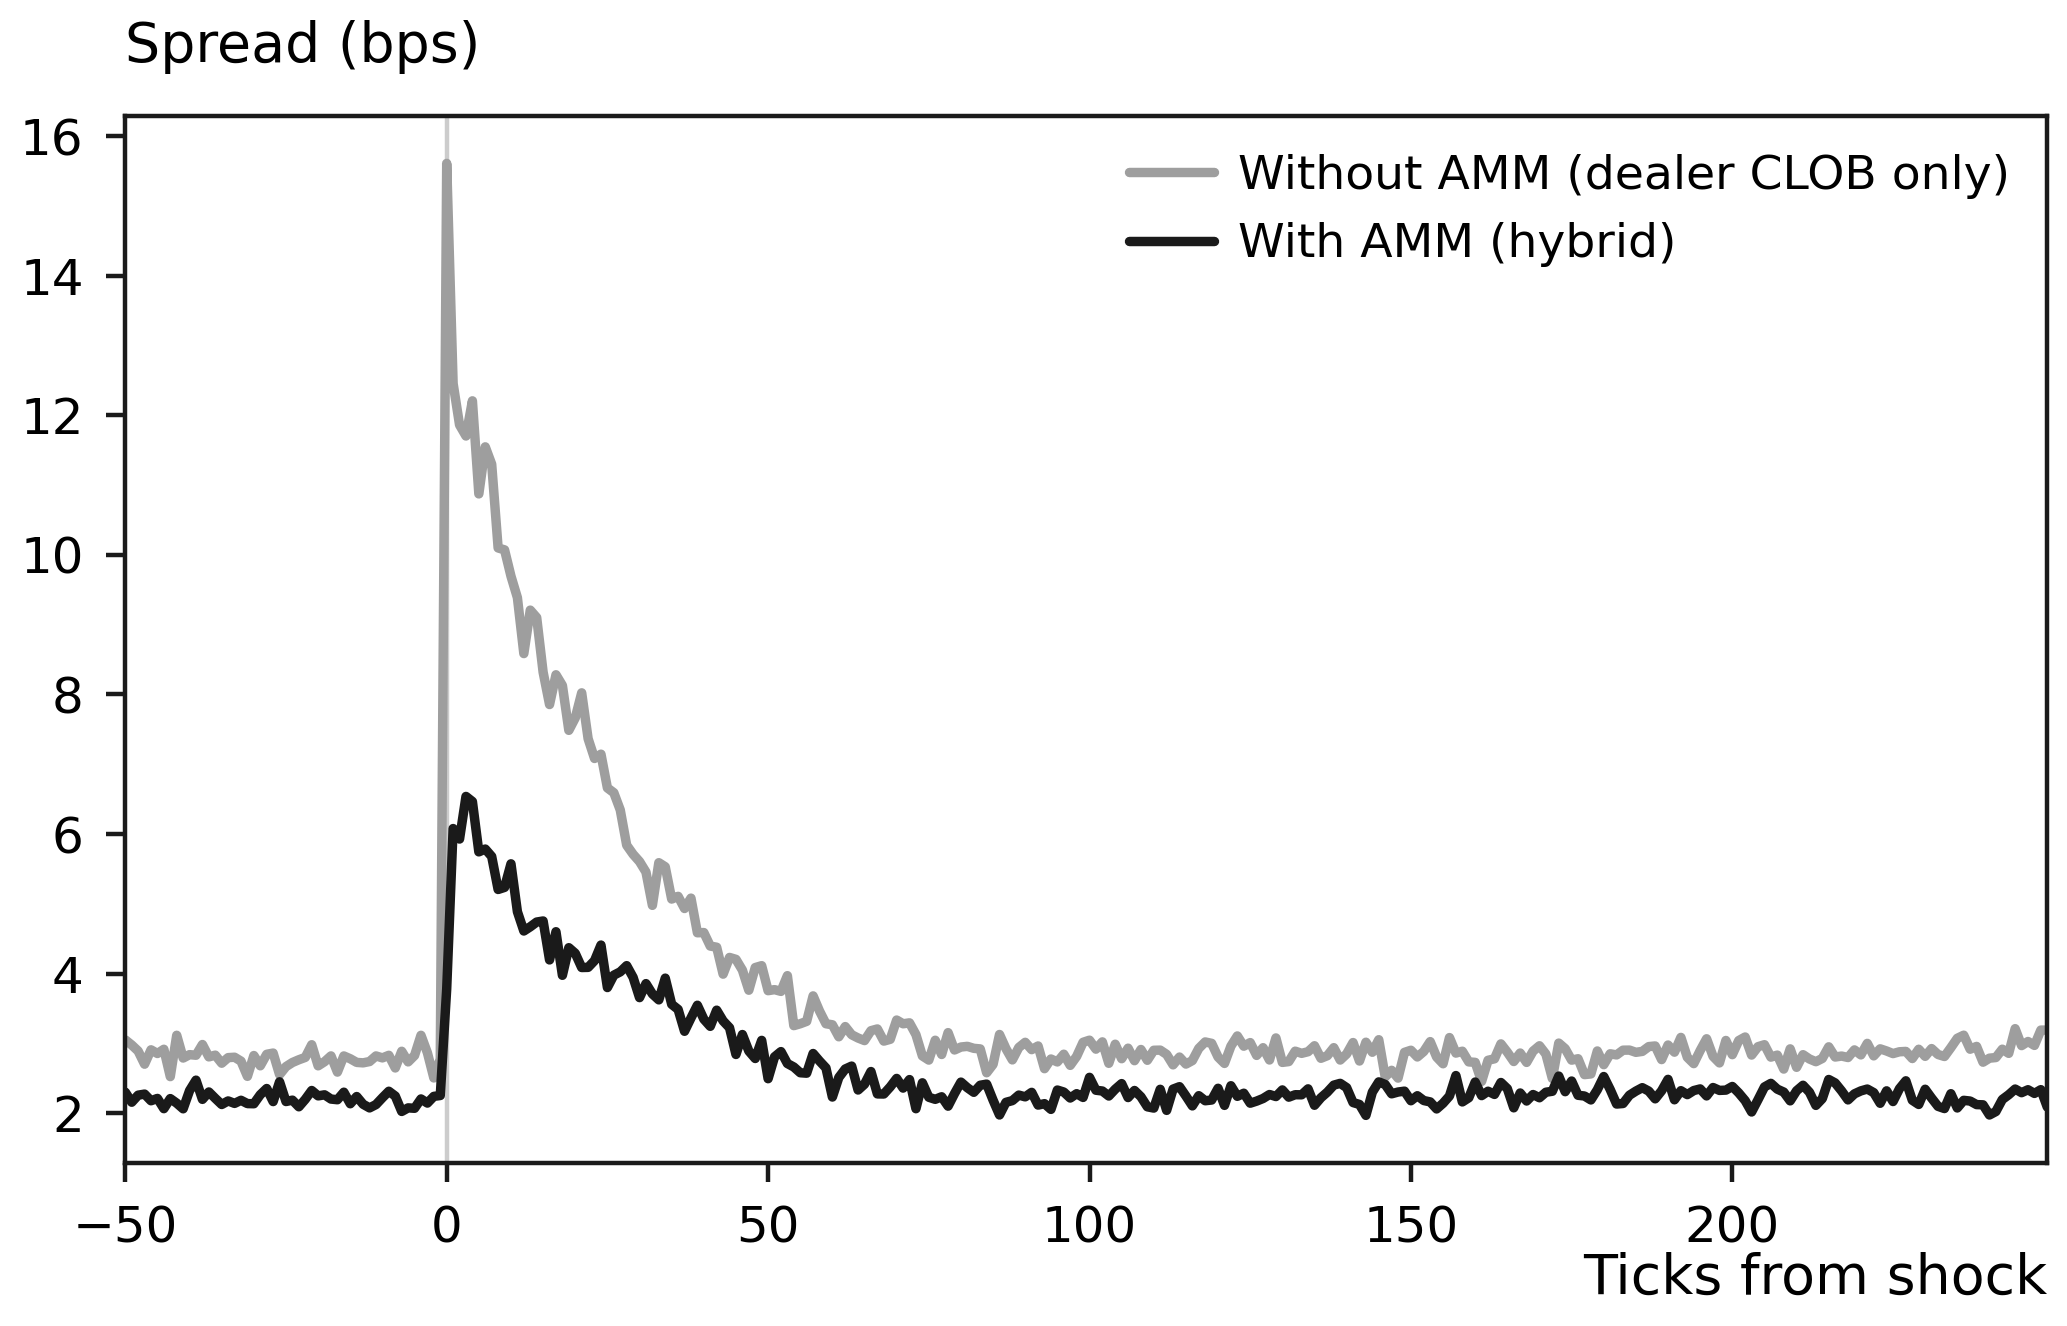
\includegraphics[width=0.8\linewidth]{dlc_spread_trajectory.png}
\captionof{figure}{Mean quoted spread trajectory around the dealer liquidity shock.}
\label{fig:trajectory}
\end{center}

Table~\ref{tab:dlc} sets the reserve priced facility against the dealer only control, which is the unmatched comparison that establishes the raw magnitude of the effect before any attempt to decompose it. It should not, however, be read as the effect of reserve based pricing.

\begin{table}[H]
\centering
\footnotesize
\caption{Dealer liquidity crisis, hybrid versus pure dealer market (300 paired seeds, medians for levels, mean paired change with bootstrap 95\% CI in brackets, paired permutation $p$-values). Level columns are medians while the change column is the mean paired difference, so a change need not equal the difference of the two median columns. Resilience is reported following \citet{large2007} as the probability that the spread returns toward its pre shock level within the window together with the half life of the excess spread normalised by its own realised peak, so that the speed component is scale free and cannot mechanically favour the arm whose peak is lower.}
\label{tab:dlc}
\resizebox{\textwidth}{!}{%
\begin{tabular}{lrrrr}
\toprule
 & With \AMM{} & Without \AMM{} & Change [95\% CI] & $p$ \\
\midrule
Peak quoted spread (bps) & 19 & 31 & $-10.8$ \,[$-12.0,-9.6$] & $<0.001$ \\
Cumulative excess spread (bps$\cdot$ticks) & 247 & 377 & $-142$ \,[$-154,-129$] & $<0.001$ \\
Calm state spread (bps) & 2.1 & 2.7 & $-0.6$ \,[$-0.7,-0.5$] & $<0.001$ \\
\midrule
\multicolumn{5}{l}{\textit{Amplitude}}\\
\quad peak excess over pre shock level (bps) & 7.1 & 13.8 & $-6.69$ \,[$-7.29,-6.01$] & $<0.001$ \\
\midrule
\multicolumn{5}{l}{\textit{Resilience, following \citet{large2007}}}\\
\quad probability of recovery in window & 1.00 & 1.00 & $0.00$ & --- \\
\quad normalised half life (ticks) & 3 & 4 & $+0.00$ \,[$-1.00,+0.00$] & n.s. \\
\quad normalised cumulative excess & 16.9 & 16.6 & $+0.33$ \,[$-1.35,+1.42$] & n.s. \\
\bottomrule
\end{tabular}%
}
\end{table}

The peak excess over the pre shock level falls from $13.8$ to $7.1$ basis points, a paired median reduction of $6.69$ basis points with a bootstrap interval of $[-7.29,-6.01]$ over the 300 paired seeds, and cumulative excess spread over the post shock window falls by a comparable proportion. The calm state spread is also tighter, so the hybrid book is better in crisis and in calm alike.

What this comparison cannot do is attribute the reduction to the pricing rule. The treatment arm carries committed capital, an obligation to remain available, and a reserve based schedule, and the difference in Table~\ref{tab:dlc} pools all three. The placebo reported in Section~\ref{sec:results} under robustness bounds the first two from one side, and Section~\ref{sec:conc} sets out the resource matched design that would separate them properly.

\subsection{H1. Recovery dynamics}

Measuring how quickly the market recovers requires a statistic that does not reward the arm whose dislocation was smaller to begin with, and a fixed absolute band fails that requirement, since an arm peaking at $7$ basis points reaches a $4$ basis point threshold sooner than one peaking at $14$ for reasons unconnected to the speed of the underlying process. We therefore follow \citet{large2007}, who measures resiliency in two parts, namely the probability that the book replenishes at all and, conditional on replenishment, the half life of the response. The half life is computed here on the excess spread normalised by its own realised peak, which is the statistic \citet{lohall2015} report and the one against which the calibration target of Table~\ref{tab:calib} is written, and the raw event time path is read alongside it in the convention of \citet{degryse2005}.

Every seed in both arms returns toward its pre shock level within the stored window, so the probability component carries no information in this setting and the comparison rests entirely on speed. Under that comparison the two arms are indistinguishable. The normalised half life is $3$ ticks with the facility and $4$ without, the paired median difference is zero with a bootstrap interval of $[-1,0]$, and the facility is the faster arm in $48.7$\% of seeds. The normalised cumulative excess, which integrates the peak aligned response and so avoids the coarse integer resolution of a half life this short, tells the same story with medians of $16.9$ and $16.6$ and a paired difference whose interval spans zero. Figure~\ref{fig:recovery} shows the two normalised responses lying almost on top of one another.

\begin{center}
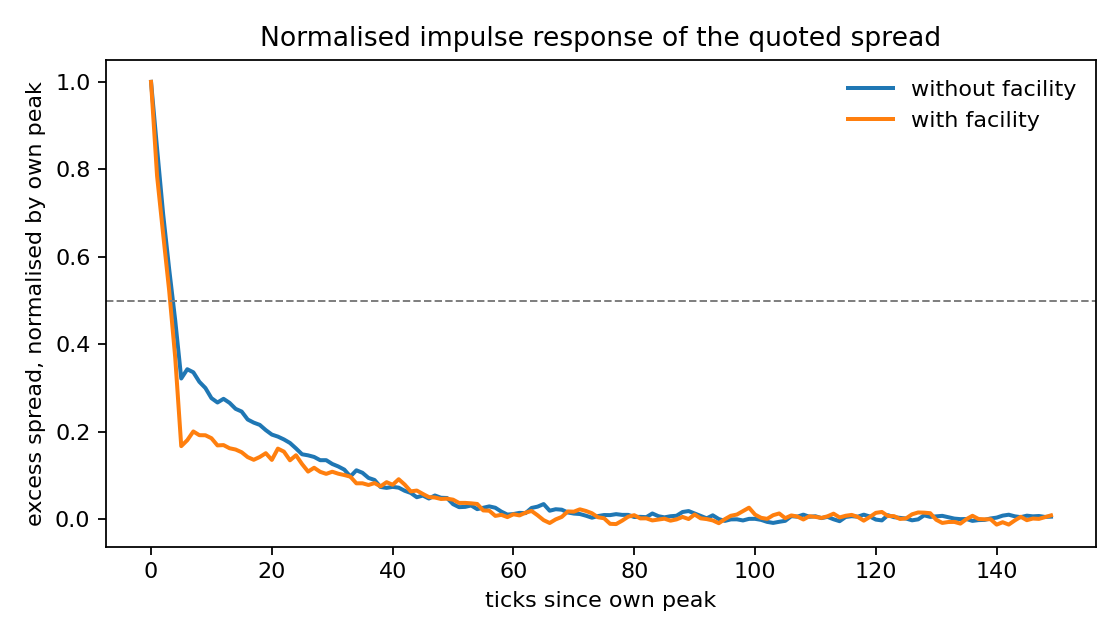
\includegraphics[width=0.8\linewidth]{recovery_normalised_irf.png}
\captionof{figure}{Normalised impulse response of the quoted spread, with each seed aligned on its own peak and scaled by it.}
\label{fig:recovery}
\end{center}

The reading we take from this is narrower than the one reported in the earlier version of this work. A standing facility lowers the amplitude of the dislocation substantially and leaves the speed at which the market works off whatever dislocation it has essentially untouched, so describing the facility as improving resilience without that qualification would restate the amplitude result in different words.

\subsection{Uncertainty}

Three distinct sources of uncertainty are reported separately, since a single interval would conflate them. Monte Carlo error describes variation across random seeds at fixed parameters and is what the paired bootstrap intervals in Table~\ref{tab:dlc} measure. Parameter uncertainty describes sensitivity to the design choices identified in Section~\ref{sec:calib} and is addressed by the sweeps below. Structural uncertainty describes dependence on the behavioural equations, the routing rule and the construction of the shock, and is not quantified by either. We therefore avoid describing any outcome as confirmatory. Small p values here indicate that a modelled difference is stable across realisations, not that the same difference would obtain in an actual crisis.

\subsection{Robustness}

The severity reduction is stable as the dealer book is deepened from five to twenty dealers, which rules out the possibility that the result depends on the knife edge fragility of a thin book.

\begin{table}[h]
\centering
\footnotesize
\caption{Dealer count sensitivity of the dealer liquidity crisis severity reduction (with minus without \AMM{}, 120 paired seeds per count, relative change in the median, all $p<0.001$).}
\label{tab:ndealer}
\begin{tabular}{lccc}
\toprule
Dealers $N$ & Peak spread & Cumulative excess & Recovery (common band) \\
\midrule
$5$  & $-31\%$ & $-34\%$ & $-31\%$ \\
$10$ & $-40\%$ & $-32\%$ & $-32\%$ \\
$20$ & $-35\%$ & $-37\%$ & $-31\%$ \\
\bottomrule
\end{tabular}
\end{table}

A placebo that disables liquidity aware routing in favour of a fixed share split still cushions the crisis significantly, which shows that standing availability does real work independently of intelligent allocation. This is the closest the present design comes to separating availability from pricing, since it indicates that a meaningful part of the effect is generic to any facility that stays open. It does not complete the separation, because the placebo arm still carries capital the control arm lacks.

The sign also survives randomizing the entire agent population across a 200 point Latin hypercube design.

\begin{table}[h]
\centering
\footnotesize
\caption{Agent composition sweep, dealer liquidity crisis. Columns report the OLS coefficient and $t$-statistic of the number of automated venues $n_{mm}$ in a regression of the with minus without \AMM{} effect on the full agent composition vector ($200$ Latin hypercube points, $188$ df), and the share of the $190$ \AMM{}-containing compositions in which the \AMM{} improves the metric. A negative coefficient on spread, cost, and volatility (and a positive one on depth) means more automated liquidity improves the metric.}
\label{tab:composition}
\begin{tabular}{lccc}
\toprule
Outcome & $\beta_{n_{mm}}$ & $t$ & \AMM{} helps (of $190$) \\
\midrule
Quoted spread (bps)      & $-0.221$              & $-5.4$ & $190/190$ \\
Execution cost ($Q{=}5$) & $-0.126$              & $-5.4$ & $190/190$ \\
Realized volatility      & $-9.0\times10^{-5}$   & $-5.7$ & $190/190$ \\
\CLOB{} depth (units)    & $+4.85$               & $+5.3$ & $184/190$ \\
\bottomrule
\end{tabular}
\end{table}

Degrading the facility oracle with a stress widening lag and noise leaves the peak spread reduction essentially unchanged, so the result does not rest on perfect pricing. A stale oracle would still worsen the price takers receive, a cost this check does not credit.

\begin{table}[h]
\centering
\footnotesize
\caption{Stale/noisy oracle robustness of the dealer liquidity crisis peak spread reduction (with minus without \AMM{}, $120$ paired seeds, sign flip permutation $p$-values, bootstrap $95$\% CIs). Only the pool oracle is degraded. Lag and noise parameters are the calm intercepts $(a_0,\eta_0)$ with their stress slopes $(k_a,k_\eta)$ in parentheses, with $\mathrm{stress}_t=\max\{\sigma_t/\sigma_0-1,3(1-\ell_t)\}$. The reduction is statistically indistinguishable across oracle quality.}
\label{tab:oracle}
\begin{tabular}{lccc}
\toprule
Oracle setting & Lag $a_0\,(+k_a)$ & Noise $\eta_0\,(+k_\eta)$ bps & Peak spread reduction \\
\midrule
Ideal (control) & --          & --        & $35.4\%$ \,[$29.2,39.5$] \\
Mild            & $0.50\,(+0.30)$ & $2\,(+5)$  & $38.1\%$ \,[$32.7,44.8$] \\
Severe          & $0.70\,(+0.50)$ & $5\,(+20)$ & $40.7\%$ \,[$33.2,43.6$] \\
\bottomrule
\end{tabular}
\end{table}

\subsection{H2. Flow migration under dealer withdrawal}

H2 concerns where the flow goes once dealers leave, and the pattern in the simulations is unambiguous, since dealers withdraw as the crisis hits and order flow migrates toward the facility. Averaged over the shock window, the facility share of executed flow rises from about 28 percent before the shock to 46 percent during it, reverting to about 30 percent afterwards, while the share of fully withdrawn dealers rises sharply. As noted in Section~\ref{sec:model}, the direction of this result follows from the routing rule. We report it because the magnitude and the speed of reversion are not determined by that rule.

\begin{table}[H]
\centering
\footnotesize
\caption{Flow migration from \CLOB{} to \AMM{} across the shock window, averaged over 300 paired seeds. \AMM{} shares are percentages of executed flow before, during, and after the shock. Here $\Delta$ is the during minus before change (pp) and the ratio is during/before. The last column is the share of the five dealers fully withdrawn during the shock, averaged over the window and seeds, with a further fraction quoting defensively at wider spreads rather than withdrawing outright. High values mark the severe, sustained crises, where the order book is then sustained by the nondealer liquidity layer and the \AMM{}. As dealers withdraw, the \AMM{} share rises in every scenario.}
\label{tab:migration}
\resizebox{\textwidth}{!}{%
\begin{tabular}{lcccccc}
\toprule
 & \multicolumn{3}{c}{\AMM{} share (\%)} & & & Dealers withdrawn \\
\cmidrule(lr){2-4}
Scenario & Before & During & After & $\Delta$ (pp) & Ratio & during (\%) \\
\midrule
Isolated dealer retreat & 27 & 36 & 28 & $+9.0$ & 1.33 & 27 \\
Flash crash & 28 & 41 & 29 & $+13.2$ & 1.48 & 44 \\
Dealer liquidity crisis & 28 & 46 & 30 & $+17.9$ & 1.64 & 86 \\
Funding shock & 27 & 46 & 31 & $+18.6$ & 1.68 & 74 \\
High volatility stress & 31 & 55 & 32 & $+23.3$ & 1.74 & 42 \\
\bottomrule
\end{tabular}%
}
\end{table}

\subsection{H3. A tail backstop, not a cheaper everyday venue}

Under H3 the facility serves the tail of the size distribution, and it does not undercut the dealer on the typical trade. Figure~\ref{fig:costsize} plots the median all in cost against trade size for both venues, in calm and at the crisis stress peak. In calm the dealer is cheaper at every size. Under stress the dealer remains cheaper for small and medium trades, but its cost rises steeply with size as the thinned book is walked while the reserve schedule barely moves, so the two cross at an intermediate size beyond which the facility is decisively cheaper.

\begin{center}
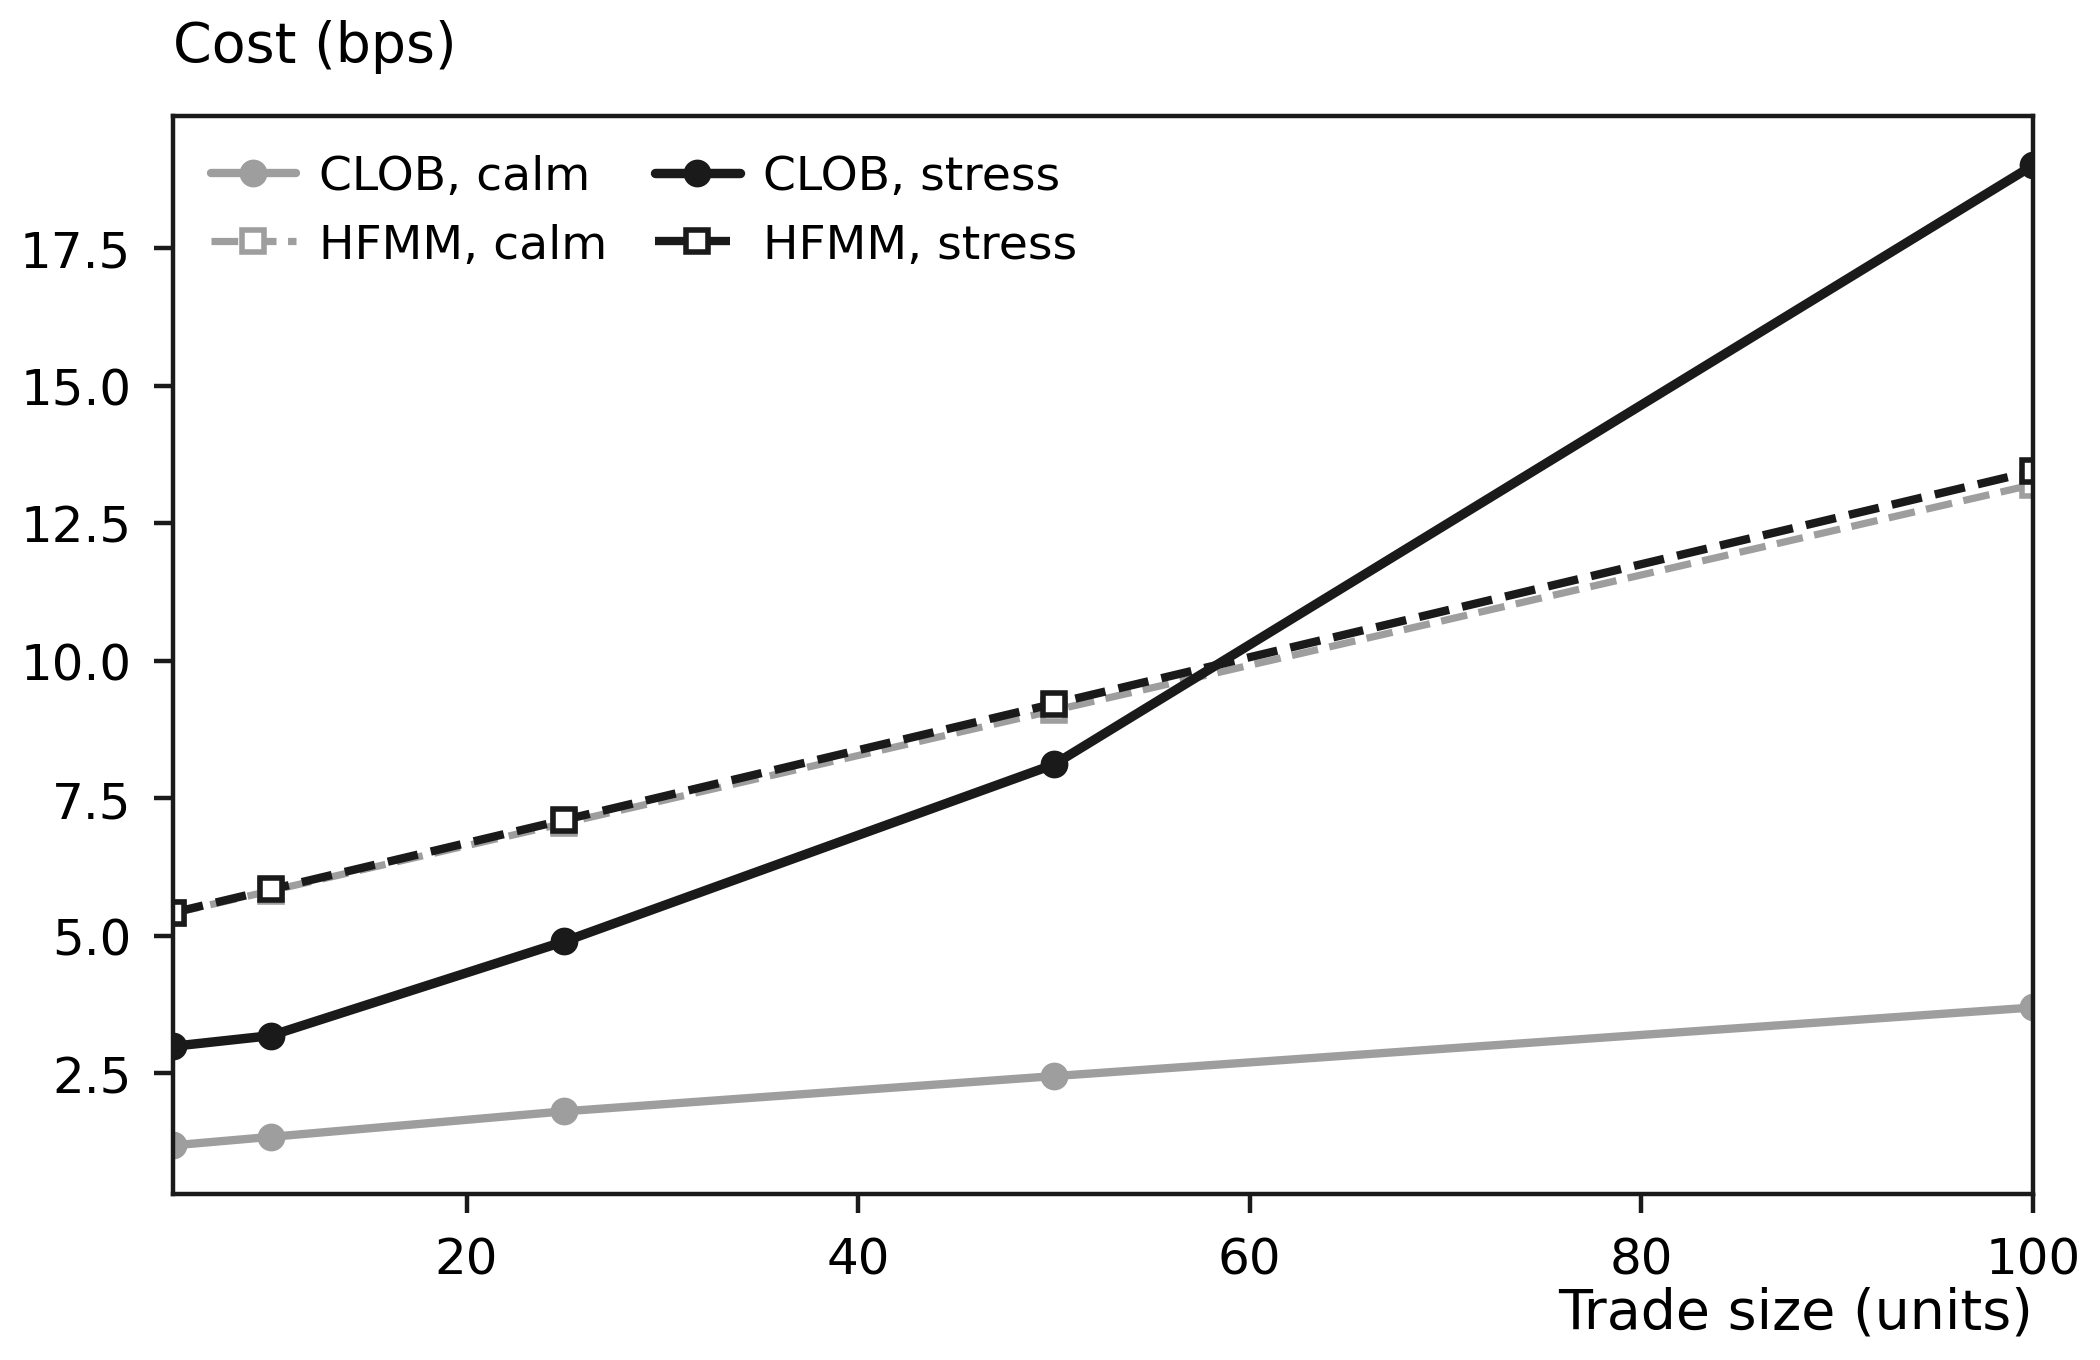
\includegraphics[width=0.8\linewidth]{dlc_cost_by_trade_size.png}
\captionof{figure}{All in execution cost versus trade size.}
\label{fig:costsize}
\end{center}

This is the clearest place where the work is done by the pricing rule and not by mere availability. A dealer of last resort quoting a single spread cannot reproduce it, because the tail advantage arises from the curvature of the schedule. The location of the crossover depends on amplification and fee, both of which are design choices, so we do not treat its exact value as a result. What is robust across the design grid is that the crossover sits well above the small and medium range.

\begin{table}[h]
\centering
\footnotesize
\caption{H3 crossover size robustness across the \AMM{} design grid (dealer liquidity crisis stress peak, $60$ seeds per cell). Entries are the median trade size in model units ($\approx$ EUR mn) at which the all in \HFMM{} cost falls below the \CLOB{} cost and stays below, with bootstrap $95$\% CIs. The crossover stays well above the $5$--$50$-unit small/medium range in every cell, rising with the fee and with curve steepness (lower $A$).}
\label{tab:crossover}
\begin{tabular}{lccc}
\toprule
 & \multicolumn{3}{c}{Pool fee} \\
\cmidrule(lr){2-4}
Amplification $A$ & $5$ bps & $10$ bps & $20$ bps \\
\midrule
$9$              & $82$ \,[$48,119$] & $122$ \,[$98,132$]  & $128$ \,[$118,138$] \\
$18$ (benchmark) & $58$ \,[$30,68$]  & $84$ \,[$74,96$]    & $112$ \,[$93,132$] \\
$36$             & $56$ \,[$40,66$]  & $88$ \,[$74,104$]   & $120$ \,[$106,136$] \\
\bottomrule
\end{tabular}
\end{table}

We read this pattern as an out of sample validation rather than as a novel claim, since \citet{barbon2023} document the same ordering empirically in a different market and our calibration never targeted it.

\subsection{Generality across stress scenarios}

\begin{center}
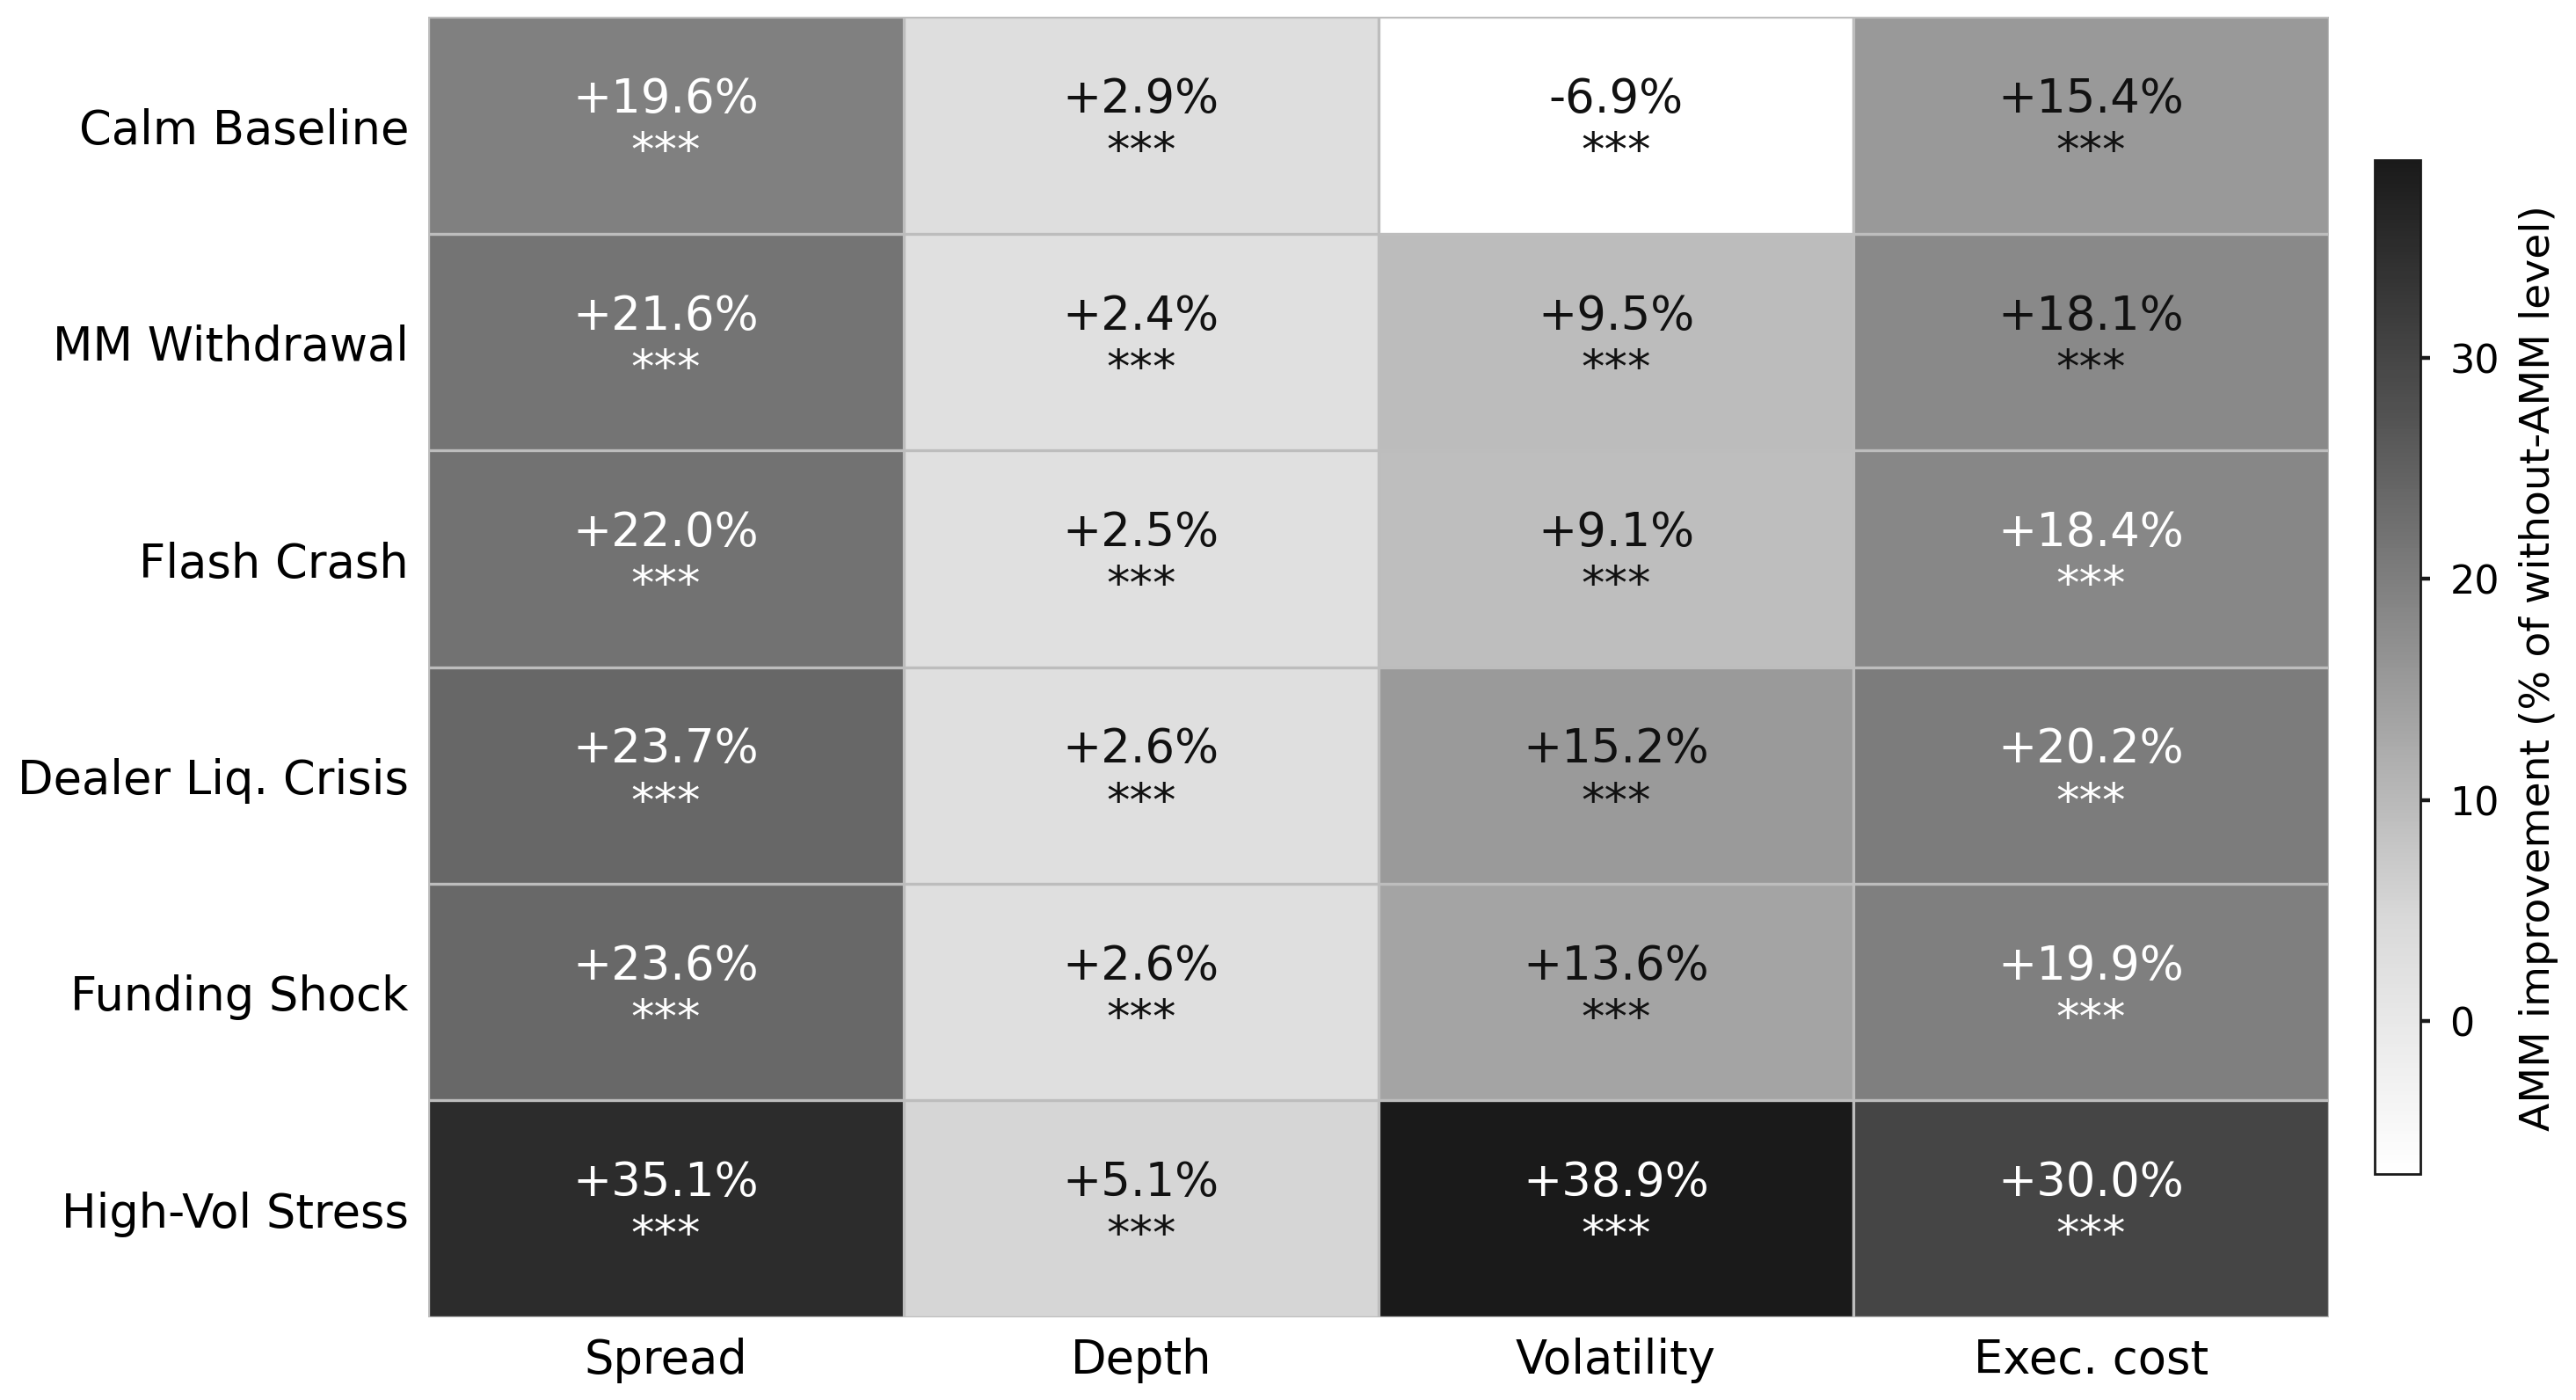
\includegraphics[width=0.95\linewidth]{shock_quality_heatmap_frl.png}
\captionof{figure}{Market quality improvement across stress scenarios.}
\label{fig:heat}
\end{center}

The improvement is positive in nearly every scenario and metric cell, materially so for spread and execution cost. Cross scenario magnitudes are indicative only, since the scenarios differ in several parameters at once, and the significance markers are descriptive and not corrected for multiple comparisons.

\section{Provider economics and welfare accounting}
\label{sec:welfare}

\subsection{Does the facility lose money}

A standing facility that loses money without compensation cannot be sustained for long, so the provider side deserves a direct answer and not a remark in passing. The answer is that the facility loses money, and that it loses more in stress than in calm.

A passive provider is arbitraged whenever the rate moves, because the reserve schedule reprices only through arbitrage and standing quotes are picked off as the price reanchors. The frictionless loss versus rebalancing benchmark of \citet{milionis2022}, applied to an amplified curve, is large, but it assumes continuous arbitrage and is therefore an upper bound. Our model caps arbitrage capacity in stress, so the realized loss is far smaller.

Marking reserves period by period against the reserves carried into that period, netting out the capital that entered or left, and crediting the fee income actually earned, the facility loses money in both windows and loses more in the crisis window than in the calm one. Raising the fee improves the provider side and weakens the backstop, since progressively less flow is routed to the facility. Magnitudes are withheld here pending re measurement, because the participation condition changes the reserves the loss is measured on, the measurement itself has been rebuilt, and the volatility of the latent price has been re anchored to a single definition of the tick. Reporting figures that three separate changes are about to move would be reporting them twice.

This fee frontier is the central tension of the design, and our treatment of it is incomplete in one specific way that should be stated plainly. \citet{hasbrouck2024dex} show that higher fees can attract inventory and thereby lower price impact, so that volume need not fall. Because committed liquidity here follows a fixed rule with a floor instead of a participation condition, that channel operates only partially, and our fee comparative static should not be read as a general result.

The facility also absorbs adversely selected flow, since the orders that migrate in stress are precisely those the dealer sector is least willing to take, and a reserve priced venue cannot defend itself by widening. This reinforces the reading of the facility as funded infrastructure whose costs are borne outside its own fee income.

\subsection{Placing the gain and the cost in a common frame}

The resilience gain accrues to the taker side as a reduction in the crisis spread and execution cost spike. The cost falls on whoever funds the facility, as a loss of a fraction of committed capital per crisis. These are measured in different units, over different populations and on different time horizons, and a direct comparison of a percentage reduction in spread with a percentage loss of pool value is not meaningful.

Expressing both sides as expected annual quantities makes them commensurable. Let \(\lambda\) denote the expected frequency of crisis episodes per year, \(V\) the committed capital, \(\ell_c\) the net provider loss per crisis window as a fraction of \(V\), and \(\ell_0\) the net loss per calm window. The expected annual cost of the facility is
\begin{equation}
\mathcal{C}(\lambda)=V\Big[\lambda \ell_c + (1-\lambda)\ell_0\Big] + r_f V \kappa,
\end{equation}
where \(r_f\) is the risk free rate and \(\kappa\) the fraction of committed capital that must be held idle, so that the second term is the opportunity cost of commitment. The expected annual benefit is the reduction in aggregate execution cost across the taker side,
\begin{equation}
\mathcal{B}(\lambda)=\lambda \sum_{Q} \omega_Q\, \Delta C(Q)\, \bar{v}_Q,
\end{equation}
where \(\omega_Q\) is the share of volume in size bucket \(Q\), \(\Delta C(Q)\) the reduction in all in cost at that size, and \(\bar{v}_Q\) crisis window volume in that bucket. The facility is favourable when \(\mathcal{B}(\lambda)>\mathcal{C}(\lambda)\).

\TODO{Populate this accounting. It requires the volume distribution by size bucket, an assumed crisis frequency with a sensitivity range, and a value for the idle capital fraction. Report the break even crisis frequency, since that is the quantity a sponsor would need to form a view on.}

The framework leaves a good deal unsettled, since it ignores tail losses beyond the simulated windows, the cost of credit, custody and settlement arrangements, and any distributional judgement about which market participants gain. We therefore refrain from characterising the subsidy as small or the trade off as favourable, and report instead the break even frequency at which the two sides balance.

\subsection{Who would operate such a facility}

The identity of the sponsor belongs to the design of the institution and not to its implementation detail. Spot \FX{} is over the counter and dealer intermediated and has no natural pool operator, so a standing facility would require a sponsor such as an exchange run utility, a settlement operator, or a central bank liquidity arrangement. Each raises questions of credit exposure, client onboarding and oracle custody that lie outside the model. If the sponsor is the dealer sector itself, the relevant counterfactual is one in which capital is reallocated instead of added, so that total capital in the market is unchanged and only its deployment differs. That counterfactual is not run here.

\section{Conclusion}
\label{sec:conc}

We have asked how much resilience a standing liquidity facility buys in a dealer intermediated \FX{} market, and whether the way it prices matters beyond the fact that it stays open.

On the first question the answer is that the gain is substantial, while on the second the present design yields only a partial answer. A placebo that keeps the facility open while allocating flow by a fixed share still cushions the crisis, so standing availability does real work on its own, and the tail confined price advantage is something a facility quoting a single spread could not reproduce. Neither observation separates the two channels cleanly, because the treatment arm carries capital the control arm does not.

Completing that separation requires a resource matched design, and we set it out here so that it can be executed and not merely assumed. Every arm would carry the same committed capital, the same inventory capacity and the same subsidy, and would differ only in pricing. A committed dealer of last resort quoting a single spread would measure the value of standing availability. A passively managed order book facility with matched capital and inventory limits would separate the venue type from the schedule. A reallocation arm, in which capital is moved out of the dealer sector instead of being added to it, would hold total market capital fixed. The difference between the reserve priced arm and the dealer of last resort arm at equal capital and equal subsidy is the quantity that identifies the contribution of the pricing rule. We report no such estimate here because those runs have not been carried out.

Three limitations bound these conclusions, the first of which concerns the supply of liquidity itself. Committed liquidity adjusts to fee income, volatility and funding cost, but through a reduced form rule with a floor beneath which the pool cannot fall, so the facility can shrink and never be abandoned, and the compensation required to retain providers is imposed instead of solved for. The fee comparative static inherits that limitation, since the mechanism of \citet{hasbrouck2024dex} works through exactly the participation margin the rule suppresses. The facility rate is pegged to the latent fair price in the baseline, with oracle degradation examined only as a robustness check. The design covers a single currency pair, so the commonality measure is weakly informative and we do not present it as a finding.

The natural next step is to replace the liquidity rule with a participation condition derived from the provider payoff, allowing providers to enter, to leave without a floor, and to be compensated at a fee the model solves for, so that the availability on which the whole result rests becomes an equilibrium outcome.

\paragraph{Reproducibility and data availability.} Each scenario is run over 300 paired seeds, base seed 42, with the arms sharing each seed and shock schedule. Code, parameter files, and seed lists are provided in a repository for review and will be deposited in a permanent public archive upon publication.

\paragraph{Funding.} This research received no specific grant from any funding agency in the public, commercial, or not for profit sectors.

\paragraph{Declaration of competing interest.} The authors declare that they have no known competing financial interests or personal relationships that could have appeared to influence the work reported in this paper.

\printcredits

\newpage
\bibliographystyle{unsrtnat}
\bibliography{refs}

\end{document}
